\documentclass[noindent, nochapname]{tudexercise}
\usepackage[utf8]{inputenc}
\usepackage[english]{babel}
\usepackage{amsmath}
\usepackage{listings}
\usepackage{booktabs}
\title{Natural Language Processing and the Web}
\subtitle{Machine Learning Project - Documentation}
\subsubtitle{Benedikt Lins (1799381) und Stefan Thaut (1800351)\\
			Department 20 - Computer Science\\
			\today}
\setlength{\parindent}{0em} 
\begin{document}
	\lstset{language=Java}
	\maketitle
	
	\section{Foundations}
		In this Machine Learning Project we want to develop a named entity recognizer based on a machine learning approach. A named entity is a set of tokens, which form a name. Examples are "New York" or "Angela Merkel". We use a Conditional Random Field as the machine learning model.\\
		Our training set contains a set of tokens with a chunk-annotation and the associated named entity class relating to the IOB-notation. We also have a german training set, that additionally contains a lemma for the given token.\\
		An analysis for the english training set shows, that about 83 \% of all tokens are no named entities, as we can see in figure \ref{fig:class_distribution}
		
		\begin{figure}[h]
			\centering
			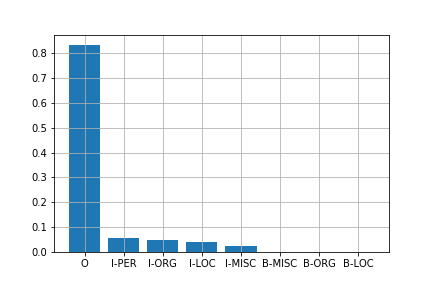
\includegraphics[scale=0.6]{img/class_distribution.png}
			\caption{Class distribution of the english training set}
			\label{fig:class_distribution}
		\end{figure}
		
		Our CRF-model is based on the CRF-model we heard about in the fifth exercise of the lecture. So we already used the provided features:
		\begin{itemize}
			\item Is the first letter of a token capitalized? (Cap)
			
			\item Number of characters (NoOfChar)
		\end{itemize}
		
		In table \ref{tab:results} we can see the improvement of the measurements with this features in comparison to the baseline. The Micro F1 is increased by about just 0.035, but the Macro F1 is increased by about 0.15.
		
		\subsection{Evaluation}
			To have a baseline for an evaluation, with which we can compare our results, we added just a dummy feature to the CRF-model and did a testrun with the english trainingset and the english validationset as testset. The evaluationmetrics are shown in table \ref{tab:results}.
			
			\begin{table}[h]
				\centering
				\caption{Evaluation results for different feature combinations}
				\label{tab:results}
				\begin{tabular}{lcc}
					\toprule
& \textbf{Micro F1} & \textbf{Macro F1}\\
					\midrule
Baseline & 0.8253 & 0.1130\\
Cap, NoOfChar & 0.8602 & 0.2693\\
ltcForO & 0.8253 & 0.1130\\
Cap, NoOfChar, ltcForO & 0.8596 & 0.2691\\
					\bottomrule
				\end{tabular}
			\end{table}
	
	\section{Additional features}
		\subsection{Last two characters of a token}
			At first we have tried to use the last two characters (ltc) of a token as a feature. For the meaningfulness of this feature, we analysed the most frequent ltc for the class \textit{O} and for the tokens, that are not in the class \textit{O}. The ten most frequent ltc are presented in figure \ref{fig:ten_most_frequent_ltc}.
			
			\begin{figure}[h]
				\centering
				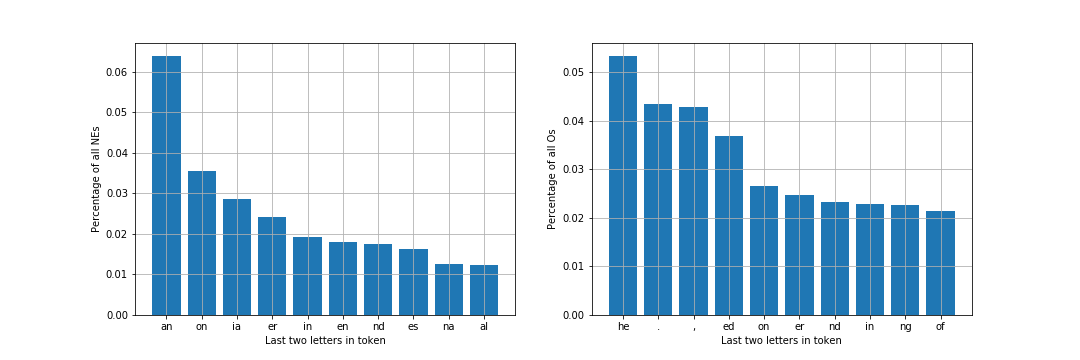
\includegraphics[scale=0.5]{img/last_two_letters_per_class.png}
				\caption{This figures show the ten most frequent ltc. The right side shows the ltc for the class \textit{O} and the left side shows the ltc for all tokens, that are not in class \textit{O}}
				\label{fig:ten_most_frequent_ltc}
			\end{figure}
			
			As we can see, about six percent of all named entities end with "an" and about five percent of all non named entities end with "he". In the next step it is important to find out, if some endings are typical for named entities or for non named entities. So we examined the appearances of the most frequent ltc of named entities in tokens that are non named entities and vice versa. The results for the ten most frequent ltc are shown in figure \ref{fig:ten_most_frequent_comparison}. The left side shows the comparison for the most frequent ltc of named entities. The blue curve represents the occurences of the ltc in named entities and the orange curve represents the occurences of the ltc in non named entities. So we can imply, that the greater the distance between the both curves is, the more specific the ltc is for the class. We identified the ltc "an", "ia", and "na" as typical for named entities and analogously the ltc "he", ".", ",", "ed" and "of" as typical for non named entities.\\
			
			\begin{figure}[h]
				\centering
				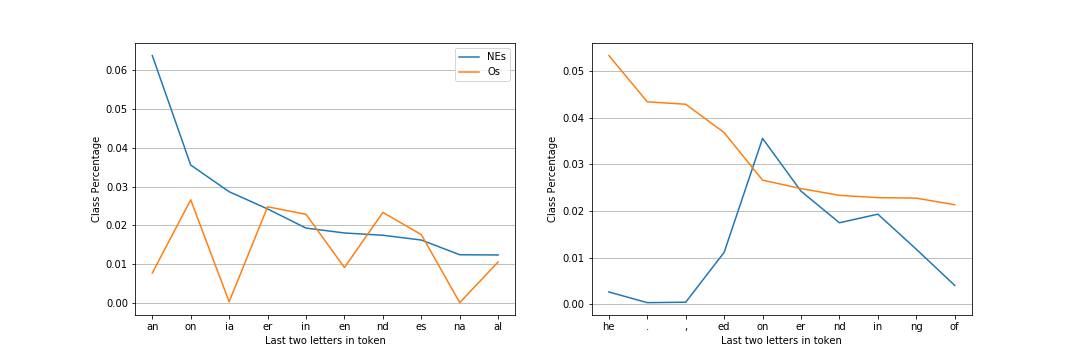
\includegraphics[scale=0.5]{img/last_two_letters_comparison.png}
				\caption{This figures show the percentages of the ten most frequent ltc in comparison of the classes named entity and non named entity}
				\label{fig:ten_most_frequent_comparison}
			\end{figure}
						
			In a first testrun with this observations, we used only the ltc, that are typical for non named entities (ltcForO). As we can see in table \ref{tab:results}, we do not get an improvement in comparison to the baseline with this new feature. When we add this features to the capital- and the number-of-char-feature, we even decrease the evaluation in comparison to the use of both of the features.\\
			
			We assumed the insufficient classification as the reason for the lower evaluation. We determined just two classes: named entities and non named entities. But there are finer classes for the named entities. So in a second step we searched for the five most frequent ltc for each class and plotted it against the frequencies of the ltc in the other classes (see figure \ref{fig:ltc_for_all_classes}). The cell for a specific ltc in a specific class is brighter, the more typical the ltc is for this class (i.e. the more token in the class end with the ltc). Thus we can use a ltc as a feature, if a cell for this ltc is nearly white or if all other cells in the column of a ltc are black (i.e. this ltc does not occur in any other class).

\end{document}